\documentclass{article}

\usepackage{graphicx}
\usepackage{tikz}
\usepackage{tikzsymbols}
\usetikzlibrary{calc,patterns,shapes.geometric}
\pagestyle{empty}
\usepackage[margin=0pt]{geometry}
\geometry{papersize={14in,12in}}

\def\centerarc[#1](#2)(#3:#4:#5){\draw[#1] ($(#2)+({#5*cos(#3)},{#5*sin(#3)})$) arc (#3:#4:#5);}

\begin{document}
	\begin{figure}
		\centering
		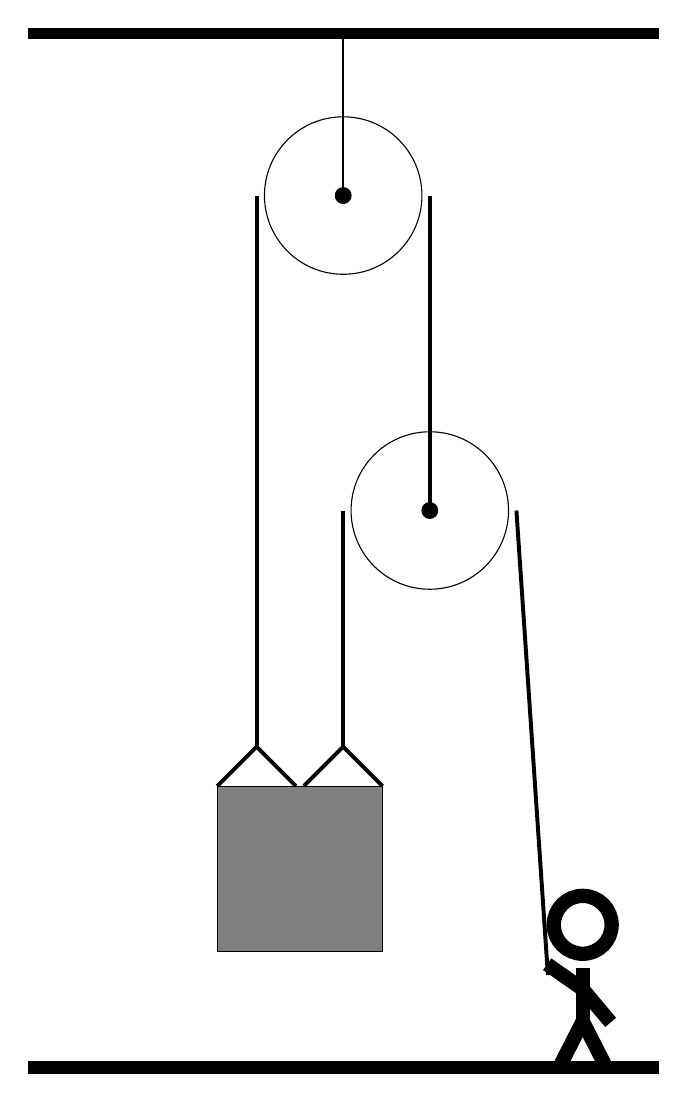
\begin{tikzpicture}
			%%%%% START %%%%%
			\draw[fill=black] (-2, 10) rectangle (6, 10.125);
			
			\draw (2, 8.0) circle (1);
			\draw[fill=black] (2, 8.0) circle (0.1);
			\draw[thick] (2, 8.0) -- (2, 10);
			
			\draw (3.1, 4.0) circle (1);
			\draw[fill=black] (3.1, 4.0) circle (0.1);
			
			\draw[line width = 0.5mm]  (0.4, 0.5) -- (0.9, 1.0) -- (1.4, 0.5);
			\draw[line width = 0.5mm]  (1.5, 0.5) -- (2.0, 1.0) -- (2.5, 0.5);
			\draw[fill=black!50] (0.4, 0.5) rectangle (2.5, -1.6);
			
			\draw[line width = 0.5mm] (0.9, 8.0) -- (0.9, 1.0);
			\centerarc[line width = 0.5mm](2, 8.0)(0:180:1.1);
			\draw[line width = 0.5mm] (3.1, 8.0) -- (3.1, 4.0);
			\draw[line width = 0.5mm] (2.0, 4.0) -- (2.0, 1.0);
			\centerarc[line width = 0.5mm](3.1, 4.0)(0:180:1.1);
			\draw[line width = 0.5mm] (4.2, 4.0) -- (4.6, -1.9);
			
			\node at (5, -2) {\Strichmaxerl[10][-35][-50]};
			
			\draw[fill=black] (-2, -3) rectangle (6, -3.15);
			%%%%% END %%%%%
		\end{tikzpicture}
	\end{figure}	
\end{document}